\listfiles
\documentclass[review]{elsarticle}

\usepackage{lineno,hyperref}
\modulolinenumbers[5]

\journal{Forensic Science International: Digital Investigation}

%%%%%%%%%%%%%%%%%%%%%%%
%% Elsevier bibliography styles
%%%%%%%%%%%%%%%%%%%%%%%
%% To change the style, put a % in front of the second line of the current style and
%% remove the % from the second line of the style you would like to use.
%%%%%%%%%%%%%%%%%%%%%%%

% Numbered
% \bibliographystyle{model1-num-names}

%% Numbered without titles
% \bibliographystyle{model1a-num-names}

%% Harvard
% \bibliographystyle{model2-names}\biboptions{authoryear}

%% Vancouver numbered
% \usepackage{numcompress}\bibliographystyle{model3-num-names}

%% Vancouver name/year
% \usepackage{numcompress}\bibliographystyle{model4-names}\biboptions{authoryear}

%% APA style
% \bibliographystyle{model5-names}\biboptions{authoryear}

%% AMA style
% \usepackage{numcompress}\bibliographystyle{model6-num-names}

%% `Elsevier LaTeX' style, distributed in TeX Live 2019
\bibliographystyle{elsarticle-num}
% \usepackage{numcompress}\bibliographystyle{elsarticle-num-names}
% \bibliographystyle{elsarticle-harv}\biboptions{authoryear}
%%%%%%%%%%%%%%%%%%%%%%%

\begin{document}

\begin{frontmatter}

\title{Bias from dataset composition in file fragment classification}

\author[mymainaddress,mysecondaryaddress]{Atila Leites Romero}
\ead{atilaromero@gmail.com}

\address[mymainaddress]{PUC}
\address[mysecondaryaddress]{Brazilian Federal Police, Av Ipiranga 1365, Porto Alegre/RS, Brazil}


%% Group authors per affiliation:
% \author{Atila Leites Romero}
% \address{Radarweg 29, Amsterdam}

%% or include affiliations in footnotes:
% \author[mymainaddress,mysecondaryaddress]{Elsevier Inc}
% \ead[url]{www.elsevier.com}

% \author[mysecondaryaddress]{Global Customer Service\corref{mycorrespondingauthor}}
% \cortext[mycorrespondingauthor]{Corresponding author}
% \ead{support@elsevier.com}

% \address[mymainaddress]{1600 John F Kennedy Boulevard, Philadelphia}
% \address[mysecondaryaddress]{360 Park Avenue South, New York}

\begin{abstract}
TODO: govdocs was an improvement

TODO: This articles shows...
\end{abstract}

\begin{keyword}
TODO\sep TODO
\end{keyword}

\end{frontmatter}

\linenumbers

\section{Introduction}

context: dissertation

first question: search for best model

\section{Related work}
The early studies on data carving used private datasets
\cite{karresand_file_2006} \cite{veenman_statistical_2007} \cite{erbacher_identification_2007} \cite{moody_sadi-statistical_2008} \cite{calhoun_predicting_2008} \cite{li_novel_2010} \cite{conti_automated_2010} \cite{kattan_gp-fileprints:_2010},
making it difficult to compare the results of different studies. In 2009, Garfinkel \textit{et al.} \cite{garfinkel_bringing_2009} published the Govdocs1 dataset with 1 million files (a small amount of those files was removed later, for legal reasons). While some of the later works on the field still use private datasets, the Govdocs1 dataset has become the most used choice in studies related to data carving. This related work summary focuses on studies on file fragment classification that used the Govdocs1 dataset from 2009 to 2019.

Depending on the objective, the focus of each study may either be whole file classification or file fragment classification. Whole file classification is generally an easier task because most file types, even those with high entropy and low compression rates, have well-structured headers, with easily recognizable patterns.

Most of the early work in this field used some form of dimensionality reduction in the input data before performing classification, as byte frequency distribution 
\cite{karresand_oscarfile_2006} \cite{harris_using_2007} \cite{amirani_new_2008} \cite{ahmed_content-based_2010} \cite{ahmed_fast_2010} \cite{sportiello_context-based_2012} \cite{amirani_feature-based_2013} \cite{qiu_new_2014} \cite{maslim_distributed_2014} \cite{ali_classification_2018}, compression rate \cite{axelsson_normalised_2010} \cite{penrose_approaches_2013}, and various statistical techniques \cite{veenman_statistical_2007} \cite{erbacher_identification_2007} \cite{moody_sadi-statistical_2008} \cite{calhoun_predicting_2008} \cite{li_novel_2010} \cite{kattan_gp-fileprints:_2010} \cite{gopal_statistical_2011}. The usage of raw bytes \footnote{raw bytes: the original bytes of the file, without conversion or dimensionality reduction} as input is recently becoming more popular \cite{hiester_file_2018} \cite{chen_file_2018} \cite{wang_sparse_2018} \cite{wang_file_2018} \cite{vulinovic_neural_2019},
especially in studies applying machine learning techniques, which seems to be a rising trend in the last ten years.

Each of the following studies chose a subset of file types from the Govdocs1 dataset, splitting this subset further into training and validation parts. The training dataset was used to train the machine learning solution to classify file fragments, while the validation dataset was used to verify how accurately the model could predict the type of the file from which the fragment was extracted from.

Axelsson \cite{axelsson_normalised_2010} used the normalized compression distance as an input feature to a kNN algorithm, picking pairs of 512-byte fragments, compressing them with the bzip2 algorithm and comparing the length of the results.
He got an average accuracy of around 34\% using 28 file types.

Fitzgerald \textit{et al.} \cite{fitzgerald_using_2012}  used an SVM classifier with various statistical measures as input features, including unigram and bigram\footnote{
    In this context, unigram is a single byte, while bigrams are sequences of two bytes.
} histogram counts, Shannon entropy, and compression length.
Omitting the first and the last fragments of each file, they got an average accuracy of 49.1\% using 24 file types.

Beebe \textit{et al.} \cite{beebe_sceadan:_2013}
compared various measures of complexity and byte frequency distributions of 512-byte fragments as input features to an SVM algorithm. They used 8 data types, txt, base64, base85, urlencoded, fat fs data, ntfs fs data, ext fs data, aes256, and
30 file types
from the Govdocs1 dataset and some other sources (19 are at least partially from the Govdocs1 dataset). They got an average accuracy of 73.4\% combining unigram and bigrams as input features.

Chen \textit{et al.} \cite{chen_file_2018}
used a Convolutional Neural Network (CNN) with five convolutional layers and 3 fully connected layers to classify fragments of 4096 bytes, converting each fragment into a 64x64 grayscale picture.
They got an average accuracy of 70.9\% using 16 file types.

Hiester \cite{hiester_file_2018} apparently was the first to use an LSTM network to perform file fragment classification. He compared the results of three types of neural networks: feedforward, convolutional, and LSTM. He used four file types from the Govdocs1 dataset.
Each bit of a 512-byte fragment was translated into two features, resulting in 8192 features per block (512*8*2). The first and last sectors of each file in the training set were discarded. In the experiments, the datasets were limited to one gigabyte to fit in memory. He got an average accuracy of 98\% using an LSTM network, 73\% using CNN, and 76\% using MLP.

Wang \textit{et al.} \cite{wang_sparse_2018} 
used sparse dictionaries for n-grams to extract features of 512-byte fragments, using this as input to an SVM classifier.
They got an average accuracy of 61.3\% using 18 file types.

Wang \textit{et al.} \cite{wang_file_2018}  
compared CNN, SVM, kNN, and XGboost, with fragments of different sizes, converting each byte to a 256-length vector (one-hot encoding). The CNN combined three parallel convolutional layers of widths 4, 8 and 16.
They used 20 file types from the Govdocs1 dataset.
Using CNN, they got an average accuracy of around 68\% with 512-byte fragments, and around 78\% with 4096-byte fragments.

Vulinović \textit{et al.} \cite{vulinovic_neural_2019}
compared a CNN with MLP, using 512 raw bytes as the CNN input, and byte histograms as input to the MLP.
Using 18 file types, they got a macro average F1-score of 61\% using CNN and 81\% using MLP.

Table \ref{tab:datacarvingstudies} summarizes 
the results of file fragment classification studies using Govdocs1 dataset and Table \ref{tab:studiesfiletypes}
lists the file types used in each study.

\begin{table*}[!ht]
\caption{\label{tab:datacarvingstudies}File fragment classification studies using the Govdocs1 dataset}
\resizebox{\linewidth}{!}{%
\begin{tabular}{|l|l|l|l|l|l|l|l|l|l|l|}
\hline
Study                                          & SVM & kNN & NN   & Dataset       & Raw   & Fragment & Number   & Accuracy   & F1-score  \\
                                               &     &     &      &               & bytes & size     & of types &            &           \\ \hline
Axelsson \cite{axelsson_normalised_2010}       &     & x   &      & Govdocs1      & No    & 512      & 28       & 34\%       &           \\ \hline
Fitzgerald \textit{et al.} \cite{fitzgerald_using_2012} & x   &     &      & Govdocs1      & No    & 512      & 24       & 49\%       & 48\%      \\ \hline
Beebe \textit{et al.} \cite{beebe_sceadan:_2013}        & x   &     &      & Govdocs1 +    & No    & 512      & 38       & 73\%       &           \\
                                               &     &     &      & other sources &       &          &          &            &           \\ \hline
Hiester \cite{hiester_file_2018}               &     &     & MLP  & Govdocs1      & Yes   & 512      & 4        & 77\%       &           \\
                                               &     &     & CNN  &               &       &          &          & 73\%       &           \\
                                               &     &     & LSTM &               &       &          &          & 98\%       &           \\ \hline
Chen \cite{chen_file_2018}                     &     &     & CNN  & Govdocs1      & Yes   & 4096     & 16       & 71\%       &           \\ \hline
Wang \cite{wang_sparse_2018}                   & x   &     &      & Govdocs1      & Yes   & 512      & 18       & 61\%       & 61\%      \\ \hline
Wang \cite{wang_file_2018}                     &     &     & CNN  & Govdocs1      & Yes   & 512      & 20       & 68\%       &           \\
                                               &     &     &      &               &       & 4096     &          & 78\%       &           \\ \hline
Vulinovic \cite{vulinovic_neural_2019}         &     &     & MLP  & Govdocs1      & Yes   & 512      & 18       &            & 81\%      \\
                                               &     &     & CNN  &               &       &          &          &            & 61\%      \\ \hline
\end{tabular}}
\end{table*}


\begin{table}[!ht]
    \centering
    \caption{The Govdocs1 dataset and file types used in each study}
    \label{tab:studiesfiletypes}
\renewcommand{\arraystretch}{0.7}
\footnotesize
\begin{tabular}{|l|l|l|l|l|l|l|l|l|l|l|l|}
\hline
Extension & Number of files & Number of blocks
                                            & \rotatebox{90}{this study}
                                                & \rotatebox{90}{Axelsson \cite{axelsson_normalised_2010}}
                                                    & \rotatebox{90}{Fitzgerald \textit{et al.} \cite{fitzgerald_using_2012}}
                                                        & \rotatebox{90}{Beebe \textit{et al.} \cite{beebe_sceadan:_2013}}
                                                            & \rotatebox{90}{Hiester \cite{hiester_file_2018}}
                                                                & \rotatebox{90}{Chen \cite{chen_file_2018}}
                                                                    & \rotatebox{90}{Wang \cite{wang_sparse_2018}}
                                                                        & \rotatebox{90}{Wang \cite{wang_file_2018}}
                                                                            & \rotatebox{90}{Vulinovic \cite{vulinovic_neural_2019}}
                                                   \\ \hline
                                                      \hline
pdf       & 231232          & 268071071     & x & x & x & x &   & x & x & x & x   \\ \hline
html      & 214568          & 25710908      & x & x & x & x &   & x & x & x & x   \\ \hline
jpg       & 109233          & 73242253      & x & x & x & x & x & x & x & x & x   \\ \hline
txt       & 78286           & 99435540      & x &   & x & x &   &   & x & x & x   \\ \hline
doc       & 76616           & 60654930      & x & x & x & x &   & x & x & x & x   \\ \hline
xls       & 62635           & 58718224      & x & x & x & x &   & x & x & x & x   \\ \hline
ppt       & 49702           & 251210471     & x & x & x & x &   & x & x & x & x   \\ \hline
gif       & 36302           & 5962516       & x & x & x & x & x & x & x & x & x   \\ \hline
xml       & 33458           & 16954875      & x & x & x & x & x & x & x & x & x   \\ \hline
ps        & 22015           & 56547464      & x & x & x & x &   &   & x & x & x   \\ \hline
csv       & 18360           & 6843009       & x & x & x & x & x & x & x & x & x   \\ \hline
gz        & 13725           & 17748905      & x & x & x & x &   & x & x & x & x   \\ \hline
log       & 9976            & 8467819       & x &   &   & x &   & x &   & x &     \\ \hline
eps       & 5191            & 5756138       & x & x &   &   &   &   &   &   &     \\ \hline
unk       & 5186            & 2983922       &   &   &   &   &   &   &   & x &     \\ \hline
png       & 4125            & 2207489       & x & x & x & x &   & x & x & x & x   \\ \hline
swf       & 3476            & 3798321       & x & x & x &   &   &   & x & x & x   \\ \hline
dbase3    & 2601            & 38972         & x &   &   &   &   &   &   & x &     \\ \hline
pps       & 1619            & 7432480       & x & x & x &   &   &   &   &   &     \\ \hline
rtf       & 1125            & 958239        & x &   & x &   &   & x & x & x & x   \\ \hline
kml       & 993             & 309422        & x &   &   &   &   &   &   &   &     \\ \hline
kmz       & 943             & 549462        & x &   &   &   &   &   &   &   &     \\ \hline
text      & 839             & 1527118       &   & x &   &   &   & x &   &   &     \\ \hline
hlp       & 659             & 8692          & x &   &   &   &   &   &   &   &     \\ \hline
f         & 602             & 94543         & x &   &   &   &   &   &   & x &     \\ \hline
sql       & 462             & 244634        & x & x & x &   &   &   &   &   &     \\ \hline
wp        & 364             & 87643         & x &   &   &   &   &   &   &   &     \\ \hline
dwf       & 299             & 85500         & x &   &   &   &   &   &   &   &     \\ \hline
java      & 292             & 14530         & x & x & x & x &   & x &   & x &     \\ \hline
pptx      & 215             & 1151796       & x & x & x & x &   &   & x &   & x   \\ \hline
% fits      & 182             & 678128        &   &   &   &   &   &   &   &   &     \\ \hline
% tmp       & 180             & 28426         &   &   &   &   &   &   &   &   &     \\ \hline
tex       & 163             & 10520         &   &   & x &   &   &   &   &   &     \\ \hline
docx      & 163             & 65969         &   & x & x & x &   & x & x &   & x   \\ \hline
% troff     & 110             & 8020          &   &   &   &   &   &   &   &   &     \\ \hline
bmp       & 72              & 62686         &   & x & x & x &   &   &   &   &     \\ \hline
% sgml      & 62              & 44138         &   &   &   &   &   &   &   &   &     \\ \hline
% gls       & 60              & 517           &   &   &   &   &   &   &   &   &     \\ \hline
pub       & 55              & 1421          &   & x &   &   &   &   &   &   &     \\ \hline
xlsx      & 37              & 12910         &   & x & x & x &   &   & x &   & x   \\ \hline
% fm        & 25              & 6717          &   &   &   &   &   &   &   &   &     \\ \hline
zip       & 10              & 31525         &   & x & x &   &   &   &   &   &     \\ \hline
ttf       & 10              & 1540          &   & x &   &   &   &   &   &   &     \\ \hline
xbm       & 8               & 578           &   & x &   &   &   &   &   &   &     \\ \hline
% wk1       & 7               & 6493          &   &   &   &   &   &   &   &   &     \\ \hline
% sys       & 7               & 15            &   &   &   &   &   &   &   &   &     \\ \hline
% ileaf     & 4               & 1656          &   &   &   &   &   &   &   &   &     \\ \hline
% exported  & 3               & 324           &   &   &   &   &   &   &   &   &     \\ \hline
% data      & 3               & 1733          &   &   &   &   &   &   &   &   &     \\ \hline
% odp       & 2               & 2384          &   &   &   &   &   &   &   &   &     \\ \hline
% mac       & 2               & 0             &   &   &   &   &   &   &   &   &     \\ \hline
% lnk       & 2               & 2             &   &   &   &   &   &   &   &   &     \\ \hline
js        & 2               & 36            &   & x &   &   &   &   &   &   &     \\ \hline
% g3        & 2               & 498           &   &   &   &   &   &   &   &   &     \\ \hline
% chp       & 2               & 73            &   &   &   &   &   &   &   &   &     \\ \hline
% 123       & 2               & 434           &   &   &   &   &   &   &   &   &     \\ \hline
% wk3       & 1               & 229           &   &   &   &   &   &   &   &   &     \\ \hline
% vrml      & 1               & 660           &   &   &   &   &   &   &   &   &     \\ \hline
% squeak    & 1               & 25354         &   &   &   &   &   &   &   &   &     \\ \hline
% py        & 1               & 480           &   &   &   &   &   &   &   &   &     \\ \hline
% pst       & 1               & 20            &   &   &   &   &   &   &   &   &     \\ \hline
% icns      & 1               & 0             &   &   &   &   &   &   &   &   &     \\ \hline
% bin       & 1               & 7             &   &   &   &   &   &   &   &   &     \\ \hline
\end{tabular}
\end{table}


As Table \ref{tab:studiesfiletypes} shows, each study on file fragment classification used a different set of file types during dataset composition. This paper explores how this seemingly minor detail may have had a major impact on results.

\section{Method}
To understand the impact that the choice of file types may have on the accuracy of a file fragment classification model, three experiments where conducted: comparison with other works, accuracy of pairs of classes, and accuracy vs. number of classes. 

\subsection{Comparison with other works}

This experiment uses a small neural network to try to replicate the results that other studies achieved using different models, by following the file type composition that each one used.

After some experimentation, a three layer neural network architecture named ``CLD'', described further ahead, was chosen to be compared with other works.

For each comparison, a new model was trained from scratch, with a dataset composed from the same file types of each of the most recent works listed in Table \ref{tab:datacarvingstudies}: 
Hiester \cite{hiester_file_2018}, 
Chen \textit{et al.} \cite{chen_file_2018},
Wang \textit{et al.} \cite{wang_sparse_2018},
Wang \textit{et al.} \cite{wang_file_2018},
and
Vulinović \textit{et al.} \cite{vulinovic_neural_2019}.
The final layer of the neural network was adjusted to match the number of file types in the set.

This comparison has three important restrictions.
Chen used 4096 bytes for the block size, while this work used 512 bytes only.
Vulinović got an F1-score\footnote{
    In binary classification problems, F1-score is the harmonic mean between precision and recall. In this context, precision is the number of true positives divided by the sum between true positives and false positives, while recall is the number of true positives divided by the sum of true positives and false negatives.
} of 81\% for the Multilayer Perceptron (MLP) fed with byte histograms, a better result than the one obtained with a Convolutional Neural Network (CNN) fed with raw bytes, 61\%. But the comparison with the ``CLD'' model of this study was based on Vulinović results with the CNN, not the MLP, because it is a more similar solution, one that uses raw bytes instead of byte histograms. Additionally, his results use F1-score, while this work measured accuracy. 

For comparison with the other two experiments, an additional model using 28 file types in the dataset composition was also trained.

\subsection{Accuracy of pairs of classes}
This experiment investigates how similar each file type is to others, to identify those that are easier to classify. 

All 378 combinations\footnote{$(28 * 27)/2 = 378$} of pairs of extensions were compared. Each pair was used to compose a dataset and to train a new model for each one. The resulting accuracy of the model should indicate if the model is able to distinguish the file types or not. An accuracy value close to 1.0 indicates that the two file types are easy to distinguish, while a value close to 0.5 indicates that the model cannot distinguish the file types, as 0.5 is the value that would be obtained by random chance.

The worst value of accuracy obtained when comparing one extension to the other 27 was used as a practical measure of how easy this extension could be classified.

Given the number of different models trained, it was important to use a model architecture that had a fast training time. Models trained with the chosen architecture took about 10 minutes to train. Without this short training period, this research step would not be feasible.

\subsection{Accuracy vs. number of classes}
This experiment uses the results of the previous experiment to explore how different dataset compositions affects the model final accuracy.

First, 135\footnote{$ 27 * 5 = 135$} independent models with the same general architecture, but different weights, were trained with 2 to 28 extensions from the Govdocs1 dataset. For each number in the range 2 to 28, a random subset of extensions was selected to compose the dataset. Each extension had 200 file samples, half placed in the training dataset and half in the validation dataset. Each dataset was used to train a new model, that should distinguish between the selected subsets of extensions in that filtered dataset. This process was repeated five times.

In a second phase, instead of randomly choosing file types, the results of the previous experiment were used to select easy to classify file types and hard to classify file types. To make that distinction, the value of the worst pair comparison of each extension was used. 

\subsection{Dataset sampling}

This study uses the Govdocs1 dataset \cite{garfinkel_bringing_2009}, which was fully downloaded and then organized by file extension.
This dataset has files with 63 different extensions. The 33 extensions with less than 200 files were discarded, to ensure the training and validation dataset would have at least 100 files of each file type.
The  ``text'' and ``unk'' extensions were discarded because examination showed that files with these extensions use multiple formats and they do not correspond to a single file type.
The remaining 28 extensions are listed in Table \ref{tab:studiesfiletypes}.

To select a sample instance from the Govdocs1 dataset, first, a random file is selected among those available, without replacement. Then, a block from this file is randomly selected. After all files have participated in the process, the process may be repeated as long as necessary. This way, all files are considered and the classes are easily balanced.
This contrasts with the sampling technique applied in other works, where all the sectors are grouped before sampling, which may lead to an imbalance between classes.

The class label used for each sample is the file type extension from where it was extracted.

The first experiment used a batch size of 300 samples, while the other two used 100 samples.

\subsection{Model}
The model architecture used in this research, referred to as``CLD'', has three layers. The first is a convolutional layer with 256 output units, a window of size 16, and a stride of 16. The second is an LSTM layer of 128 units. The last is a fully-connected layer where the number of output units matches the number of classes of the input dataset.

%optimization
All the training sessions used the Adam \cite{kingma_adam:_2014}
optimization algorithm to guide backpropagation and categorical cross-entropy as the loss function.

% Constraints
In the first experiment, the models were trained until no further improvement was observed in the last 20 epochs. In the other two experiments, this threshold was decreased to 10 epochs.

\subsection{Inputs}
The input features of the neural network for each instance are a 512x256 matrix representing only one block of 512 bytes of a random file of the dataset. Each of the 512 bytes is one-hot encoded, meaning that its value is converted into a vector with 256 elements, with only one of them set to 1, corresponding to the value of the byte, while the others are set to zero.

\subsection{Outputs}
The output of the neural network for a given instance is a vector with a size equal to the number of classes, subject to a softmax function, which applies the exponential function on the vector and then normalizes it. Each value will represent the predicted probability that the instance belongs to a specific class.

\subsection{Hardware and software}
The main software and frameworks used to build the experiments were Python 3.6 
\cite{rossum_python_2019}, Jupyter notebook \cite{perez_jupyter_2019}, Tensorflow 1.14.0 \cite{google_brain_tensorflow_2019}, Keras 2.2.4-tf \cite{chollet_keras_2019}, and Fedora Linux 27.
% repository
The source code for the experiments is available at \sloppy\url{http://github.com/atilaromero/carving-experiments}.

% \levelB{Hardware}
The experiments did not take advantage of GPU acceleration and were  conducted on a single computer with 256GB of RAM and with 2 Intel\textregistered Xeon\textregistered E5-2630 v2 processors, with 6 cores each, with 2 hyper-threads per core, or 24 hyper-threads in total. 



\section{Results}
\subsection{Comparison with other works}

Using the same file types of other works, the ``CLD'' model achieved an accuracy of 
67\% for the file types from Chen \textit{et al.} \cite{chen_file_2018},
91\% for Hiester \cite{hiester_file_2018}, 
59\% for Wang \textit{et al.} \cite{wang_sparse_2018},
65\% for Wang \textit{et al.} \cite{wang_file_2018},
and
61\% for Vulinović \textit{et al.} \cite{vulinovic_neural_2019}.

The accuracy obtained for the dataset including 28 file types was 63\%.

The results can be seen in Figure \ref{fig:cldothers}, in which the bar plot shows the comparison between the validation accuracy obtained with ``CLD'' and those achieved in other studies.

\noindent
\begin{figure*}[htb!]
\centering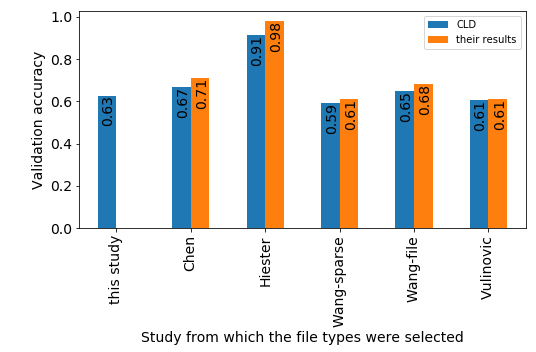
\includegraphics[width=0.8\textwidth]{CLD-others.png}
\caption[CLD vs. other studies]{\label{fig:cldothers}The ``CLD'' model was trained from scratch using the same file types used in other works. The bar plot shows the comparison between the validation accuracy obtained with ``CLD'' and those achieved in other studies. It is interesting to note that changing the dataset file type composition allowed the ``CLD'' model to achieve results similar to those of other works, despite their broad range of values. This suggests that file type composition had a bigger role than model architecture in these results.}%
\end{figure*}

\subsection{Accuracy of pairs of classes}

The data obtained comparing each pair of file types is shown in Table \ref{tab:pcadata}. The comparison of each file type with itself was not performed, but for consistency it was manually filled in the table with the value 0.5.

Figure \ref{fig:dual} shows the graph of the accuracy of each class when compared individually with each one of the others, resulting in 378 models, one for each possible pair of classes. File types where all the points are close to 100\% are hardly mistaken for other types, while accuracy values close to 50\% are the worse results possible, as they are close to random chance.

The results were organized in descending order, using the minimum accuracy result for each file type: pps, ppt, gz, png, dwf, swf, pptx, kmz, jpg, pdf, eps, ps, f, txt, gif, html, xml, doc, xls, sql, hlp, log, kml, java, csv, wp, rtf, dbase3.

\noindent
\begin{figure*}[htb!]
\centering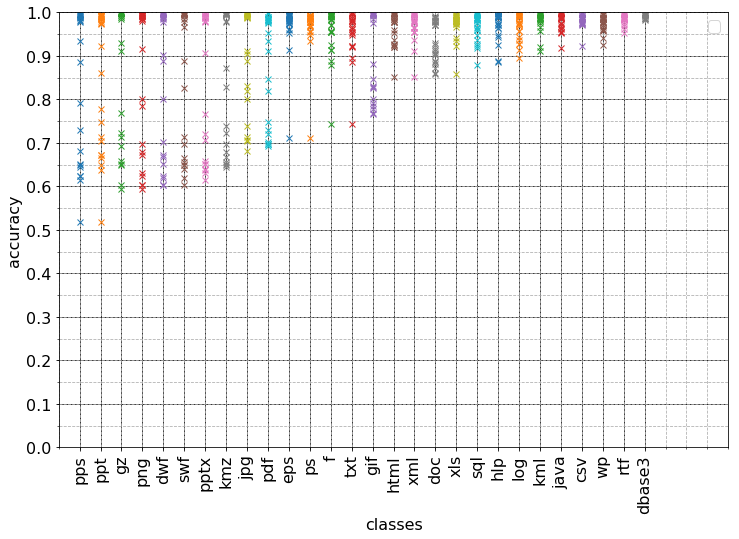
\includegraphics[width=0.8\textwidth]{dual.png}
\caption{\label{fig:dual}Validation accuracy of models trained with pair of classes. File types on the left are assumed to be harder to classify than file types on the right. Later, in the third experiment, this order will be used to select which file types will compose the dataset.}%
\end{figure*}

\begin{table}[!ht]
    \centering
    \caption[Data obtained comparing each pair of file types]{Data obtained comparing each pair of file types}
    \label{tab:pcadata}
                \rotatebox{90}{
    \renewcommand{\arraystretch}{0.8}
    \footnotesize
    \setlength\tabcolsep{1.5pt}
    \begin{tabular}{|l|l|l|l|l|l|l|l|l|l|l|l|l|l|l|l|l|l|l|l|l|l|l|l|l|l|l|l|l|}
    \hline
           & csv  & dbase3 & doc  & dwf  & eps  & f    & gif  & gz   & hlp  & html & java & jpg  & kml  & kmz  & log  & pdf  & png  & pps  & ppt  & pptx & ps   & rtf  & sql  & swf  & txt  & wp   & xls  & xml  \\ \hline
    csv    & 0.50 & 1.00   & 0.99 & 1.00 & 0.98 & 0.97 & 1.00 & 1.00 & 0.98 & 0.98 & 0.97 & 1.00 & 0.98 & 1.00 & 0.97 & 1.00 & 1.00 & 1.00 & 1.00 & 1.00 & 0.99 & 0.99 & 0.98 & 1.00 & 0.92 & 0.99 & 0.99 & 0.98 \\ \hline
    dbase3 & 1.00 & 0.50   & 0.99 & 1.00 & 1.00 & 1.00 & 1.00 & 1.00 & 0.99 & 0.99 & 0.99 & 1.00 & 0.99 & 1.00 & 1.00 & 1.00 & 1.00 & 1.00 & 0.99 & 1.00 & 0.99 & 1.00 & 0.98 & 1.00 & 1.00 & 1.00 & 0.99 & 1.00 \\ \hline
    doc    & 0.99 & 0.99   & 0.50 & 0.90 & 0.98 & 0.97 & 0.88 & 0.93 & 0.97 & 0.98 & 0.99 & 0.90 & 0.98 & 0.87 & 0.99 & 0.91 & 0.92 & 0.89 & 0.86 & 0.91 & 0.97 & 0.99 & 0.98 & 0.89 & 0.98 & 0.93 & 0.86 & 0.98 \\ \hline
    dwf    & 1.00 & 1.00   & 0.90 & 0.50 & 1.00 & 0.99 & 0.80 & 0.60 & 1.00 & 1.00 & 1.00 & 0.89 & 1.00 & 0.67 & 0.99 & 0.70 & 0.60 & 0.62 & 0.67 & 0.65 & 0.98 & 1.00 & 0.99 & 0.62 & 1.00 & 0.99 & 0.98 & 1.00 \\ \hline
    eps    & 0.98 & 1.00   & 0.98 & 1.00 & 0.50 & 0.91 & 1.00 & 0.99 & 0.99 & 0.98 & 0.99 & 0.99 & 1.00 & 0.99 & 0.98 & 0.95 & 0.99 & 0.98 & 0.97 & 0.99 & 0.71 & 0.96 & 0.96 & 0.99 & 0.98 & 0.99 & 0.98 & 0.98 \\ \hline
    f      & 0.97 & 1.00   & 0.97 & 0.99 & 0.91 & 0.50 & 1.00 & 1.00 & 0.89 & 0.93 & 0.95 & 0.99 & 0.99 & 0.99 & 0.91 & 0.99 & 0.99 & 1.00 & 0.99 & 0.99 & 0.96 & 0.99 & 0.88 & 1.00 & 0.74 & 0.96 & 0.98 & 0.95 \\ \hline
    gif    & 1.00 & 1.00   & 0.88 & 0.80 & 1.00 & 1.00 & 0.50 & 0.77 & 1.00 & 1.00 & 1.00 & 0.83 & 1.00 & 0.83 & 0.99 & 0.85 & 0.78 & 0.79 & 0.78 & 0.77 & 0.99 & 1.00 & 0.99 & 0.83 & 1.00 & 0.98 & 0.97 & 1.00 \\ \hline
    gz     & 1.00 & 1.00   & 0.93 & 0.60 & 0.99 & 1.00 & 0.77 & 0.50 & 1.00 & 1.00 & 1.00 & 0.91 & 1.00 & 0.72 & 1.00 & 0.69 & 0.59 & 0.65 & 0.71 & 0.66 & 0.98 & 0.99 & 1.00 & 0.65 & 1.00 & 0.99 & 0.99 & 1.00 \\ \hline
    hlp    & 0.98 & 0.99   & 0.97 & 1.00 & 0.99 & 0.89 & 1.00 & 1.00 & 0.50 & 0.93 & 0.96 & 0.99 & 0.99 & 1.00 & 0.94 & 1.00 & 0.99 & 0.99 & 0.99 & 0.99 & 0.99 & 0.99 & 0.95 & 1.00 & 0.89 & 0.97 & 0.97 & 0.96 \\ \hline
    html   & 0.98 & 0.99   & 0.98 & 1.00 & 0.98 & 0.93 & 1.00 & 1.00 & 0.93 & 0.50 & 0.95 & 1.00 & 0.92 & 1.00 & 0.93 & 0.99 & 0.99 & 0.99 & 0.99 & 1.00 & 0.98 & 0.98 & 0.94 & 1.00 & 0.92 & 0.96 & 0.98 & 0.85 \\ \hline
    java   & 0.97 & 0.99   & 0.99 & 1.00 & 0.99 & 0.95 & 1.00 & 1.00 & 0.96 & 0.95 & 0.50 & 1.00 & 0.98 & 1.00 & 0.97 & 0.99 & 1.00 & 1.00 & 0.99 & 1.00 & 0.99 & 0.99 & 0.92 & 1.00 & 0.96 & 0.98 & 1.00 & 0.96 \\ \hline
    jpg    & 1.00 & 1.00   & 0.90 & 0.89 & 0.99 & 0.99 & 0.83 & 0.91 & 0.99 & 1.00 & 1.00 & 0.50 & 1.00 & 0.74 & 0.99 & 0.82 & 0.80 & 0.68 & 0.70 & 0.71 & 0.99 & 1.00 & 1.00 & 0.71 & 1.00 & 0.99 & 0.99 & 1.00 \\ \hline
    kml    & 0.98 & 0.99   & 0.98 & 1.00 & 1.00 & 0.99 & 1.00 & 1.00 & 0.99 & 0.92 & 0.98 & 1.00 & 0.50 & 1.00 & 0.96 & 0.98 & 0.99 & 0.99 & 0.99 & 1.00 & 0.99 & 0.99 & 0.99 & 1.00 & 0.97 & 1.00 & 0.99 & 0.91 \\ \hline
    kmz    & 1.00 & 1.00   & 0.87 & 0.67 & 0.99 & 0.99 & 0.83 & 0.72 & 1.00 & 1.00 & 1.00 & 0.74 & 1.00 & 0.50 & 0.99 & 0.70 & 0.68 & 0.64 & 0.65 & 0.65 & 0.98 & 1.00 & 1.00 & 0.66 & 1.00 & 0.99 & 0.98 & 1.00 \\ \hline
    log    & 0.97 & 1.00   & 0.99 & 0.99 & 0.98 & 0.91 & 0.99 & 1.00 & 0.94 & 0.93 & 0.97 & 0.99 & 0.96 & 0.99 & 0.50 & 0.98 & 1.00 & 0.99 & 1.00 & 0.99 & 0.96 & 0.97 & 0.93 & 1.00 & 0.89 & 0.98 & 0.97 & 0.94 \\ \hline
    pdf    & 1.00 & 1.00   & 0.91 & 0.70 & 0.95 & 0.99 & 0.85 & 0.69 & 1.00 & 0.99 & 0.99 & 0.82 & 0.98 & 0.70 & 0.98 & 0.50 & 0.70 & 0.73 & 0.75 & 0.72 & 0.93 & 0.99 & 0.98 & 0.70 & 0.98 & 0.98 & 0.98 & 0.98 \\ \hline
    png    & 1.00 & 1.00   & 0.92 & 0.60 & 0.99 & 0.99 & 0.78 & 0.59 & 0.99 & 0.99 & 1.00 & 0.80 & 0.99 & 0.68 & 1.00 & 0.70 & 0.50 & 0.62 & 0.67 & 0.63 & 0.98 & 1.00 & 0.99 & 0.60 & 0.99 & 0.98 & 0.98 & 1.00 \\ \hline
    pps    & 1.00 & 1.00   & 0.89 & 0.62 & 0.98 & 1.00 & 0.79 & 0.65 & 0.99 & 0.99 & 1.00 & 0.68 & 0.99 & 0.64 & 0.99 & 0.73 & 0.62 & 0.50 & 0.52 & 0.61 & 0.98 & 0.99 & 0.99 & 0.65 & 1.00 & 0.98 & 0.93 & 1.00 \\ \hline
    ppt    & 1.00 & 0.99   & 0.86 & 0.67 & 0.97 & 0.99 & 0.78 & 0.71 & 0.99 & 0.99 & 0.99 & 0.70 & 0.99 & 0.65 & 1.00 & 0.75 & 0.67 & 0.52 & 0.50 & 0.64 & 0.99 & 0.98 & 0.97 & 0.66 & 0.98 & 0.97 & 0.92 & 0.99 \\ \hline
    pptx   & 1.00 & 1.00   & 0.91 & 0.65 & 0.99 & 0.99 & 0.77 & 0.66 & 0.99 & 1.00 & 1.00 & 0.71 & 1.00 & 0.65 & 0.99 & 0.72 & 0.63 & 0.61 & 0.64 & 0.50 & 0.99 & 1.00 & 0.99 & 0.64 & 0.98 & 0.98 & 0.98 & 0.99 \\ \hline
    ps     & 0.99 & 0.99   & 0.97 & 0.98 & 0.71 & 0.96 & 0.99 & 0.98 & 0.99 & 0.98 & 0.99 & 0.99 & 0.99 & 0.98 & 0.96 & 0.93 & 0.98 & 0.98 & 0.99 & 0.99 & 0.50 & 0.97 & 0.97 & 0.98 & 0.95 & 0.98 & 0.99 & 0.99 \\ \hline
    rtf    & 0.99 & 1.00   & 0.99 & 1.00 & 0.96 & 0.99 & 1.00 & 0.99 & 0.99 & 0.98 & 0.99 & 1.00 & 0.99 & 1.00 & 0.97 & 0.99 & 1.00 & 0.99 & 0.98 & 1.00 & 0.97 & 0.50 & 0.98 & 1.00 & 0.95 & 0.98 & 0.99 & 0.98 \\ \hline
    sql    & 0.98 & 0.98   & 0.98 & 0.99 & 0.96 & 0.88 & 0.99 & 1.00 & 0.95 & 0.94 & 0.92 & 1.00 & 0.99 & 1.00 & 0.93 & 0.98 & 0.99 & 0.99 & 0.97 & 0.99 & 0.97 & 0.98 & 0.50 & 1.00 & 0.92 & 0.96 & 0.99 & 0.96 \\ \hline
    swf    & 1.00 & 1.00   & 0.89 & 0.62 & 0.99 & 1.00 & 0.83 & 0.65 & 1.00 & 1.00 & 1.00 & 0.71 & 1.00 & 0.66 & 1.00 & 0.70 & 0.60 & 0.65 & 0.66 & 0.64 & 0.98 & 1.00 & 1.00 & 0.50 & 0.99 & 0.99 & 0.97 & 1.00 \\ \hline
    txt    & 0.92 & 1.00   & 0.98 & 1.00 & 0.98 & 0.74 & 1.00 & 1.00 & 0.89 & 0.92 & 0.96 & 1.00 & 0.97 & 1.00 & 0.89 & 0.98 & 0.99 & 1.00 & 0.98 & 0.98 & 0.95 & 0.95 & 0.92 & 0.99 & 0.50 & 0.96 & 0.98 & 0.96 \\ \hline
    wp     & 0.99 & 1.00   & 0.93 & 0.99 & 0.99 & 0.96 & 0.98 & 0.99 & 0.97 & 0.96 & 0.98 & 0.99 & 1.00 & 0.99 & 0.98 & 0.98 & 0.98 & 0.98 & 0.97 & 0.98 & 0.98 & 0.98 & 0.96 & 0.99 & 0.96 & 0.50 & 0.94 & 0.97 \\ \hline
    xls    & 0.99 & 0.99   & 0.86 & 0.98 & 0.98 & 0.98 & 0.97 & 0.99 & 0.97 & 0.98 & 1.00 & 0.99 & 0.99 & 0.98 & 0.97 & 0.98 & 0.98 & 0.93 & 0.92 & 0.98 & 0.99 & 0.99 & 0.99 & 0.97 & 0.98 & 0.94 & 0.50 & 0.98 \\ \hline
    xml    & 0.98 & 1.00   & 0.98 & 1.00 & 0.98 & 0.95 & 1.00 & 1.00 & 0.96 & 0.85 & 0.96 & 1.00 & 0.91 & 1.00 & 0.94 & 0.98 & 1.00 & 1.00 & 0.99 & 0.99 & 0.99 & 0.98 & 0.96 & 1.00 & 0.96 & 0.97 & 0.98 & 0.50 \\ \hline
    \end{tabular}
    }
\end{table}


\subsection{Accuracy vs. number of classes}

% decrease in accuracy
The results of the accuracy versus number of classes experiment are shown in Figure \ref{fig:nclasses}.  Each point in the graph is the validation accuracy of a distinct model trained with the indicated number of classes. The class for a block sample is the file extension of the original file. 

The ``models trained with many classes'' are the 135 results obtained by using a random selection of file types to compose the dataset.

The ``models trained with 2 classes'' are the 378 results obtained in the previous experiment, using transparency to improve visualization, as many of them are too close. 

The smooth ``random chance''line in the bottom indicates for comparison how accurate a random guess classifier would be.

% For 2 classes, the accuracy values are between 50\% and 100\%, with a greater concentration near 100\%. For 28 classes, the accuracy values are between 55\% and 58\%.

The lines ``hard file types first'' and ``easy file types first'' were created by selecting the file types that would compose the dataset. The selection was based on the results described in the previous experiment, ``Accuracy of pairs of classes'', ordering the file types by their minimum accuracy values and following this order to choose file types. For example, the ``hard file types first'' point for three classes was obtained by training a model with the file types ``pps'', ``ppt'', and ``gz'', the three classes with lower minima in Figure \ref{fig:dual}.

\noindent
\begin{figure*}[htb!]
\centering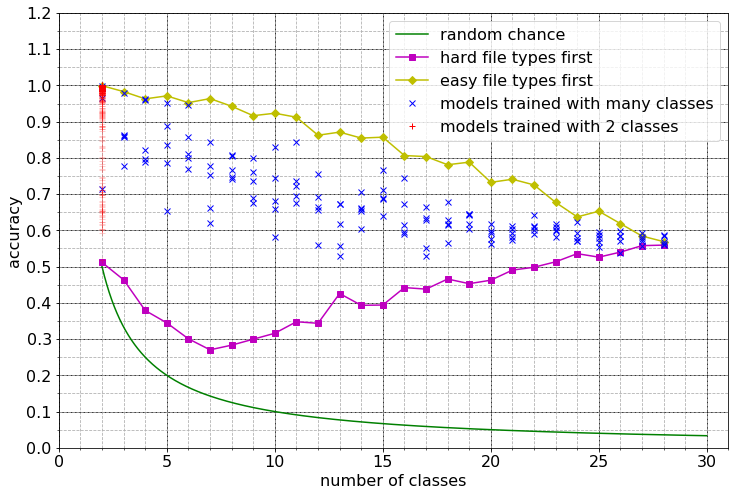
\includegraphics[width=0.8\textwidth]{nclasses.png}
\caption{\label{fig:nclasses}Validation accuracy by number of classes. This graph shows how the choice of the file types composing the dataset influences the validation accuracy of the model. A random choice of file types (the ``models trained with many classes'' line) may seem to yield an accuracy that decreases linearly with the number of classes. But this would be an incomplete conclusion, as not all file types have the same impact on accuracy. This is shown in the lines 
``hard file types first'' and ``easy file types first''. Using a carefully chosen set of file types, is possible to raise or decrease the model accuracy. For example, a model trained with the 15 file types that were considered harder had an accuracy of 39\%, while  a similar model trained with the 15 file types considered easiest had an accuracy of 85\%.}%
\end{figure*}



\section{Discussion}
A comparison was made between a chosen model, ``CLD'', and recent works in the field. While ``CLD'' achieved slight lower accuracy values than the other studies, it can be noticed that the values are similar:
while the result values of these other works range from 61\% to 98\%, a difference of 37\%, the differences between the results from this study and theirs do not exceed 7\%. This is an indication that the high  variability that these studies show between each other is caused by the difference in the file types they choose.

It was demonstrated that the accuracy of a new model may be controlled by selecting the file types that will compose the dataset. 
Some file types when included in the experiment have a much higher negative impact than others. This observation was demonstrated in the ``hard file types first'' and ``easy file types first'' of Figure \ref{fig:nclasses}, where the file types selected to compose the dataset were intentionally chosen, once to degrade results and once to improve them.

% These results highlight the importance of the file types chosen to compose the dataset and explain why the ``CLD'' model was able to almost match the results of previous works in the field, even thought they have achieved different results, as shown in Figure \ref{fig:cldothers}: the difference in choices of file types had a higher impact than the choices of models.

It is important to emphasize that the validity of the experiments of the analysed studies is not in question, since within each study the comparisons use a fixed set of file types. The problem arises only when comparisons are made between different studies.

The Govdocs1 dataset brought an important basis to compare different carving solutions. But the main conclusion of this paper is that to fairly compare results of different studies in file fragment classification, the exact same set of file types used in the original study must be first replicated.


\section{Conclusion}
Answering the second research question ``\textbf{How does the accuracy of neural network models changes relative to the number of classes in file fragment classification?}'', 
it was observed that an increase in the number of extensions selected to compose the training tends to decrease accuracy and to decrease variation in results. But the number of classes alone is not as important as the type of extension selected: some file types when included in the experiment have a much higher negative impact than others. This observation was demonstrated in the ``hard file types first'' and ``easy file types first'' of Figure \ref{fig:nclasses}, where the file types selected to compose were intentionally chosen, once to degrade results and once to improve them.


File types that contain images or that use compression were identified as those that have the highest negative effect on results, which suggests that their entropy may contribute to the error.

% \levelB{Limitations, threats to validity and future work}
The number of samples taken was small when compared to the number of all possible file types combinations. This imposes a limit on the conclusions that can be reached, and this limitation is hard to overcome.

The group that emerged as file types that most degrade results are files that use compression or contain images. While they are known for their high entropy, no measure of entropy was used to reinforce this claim.
This aspect is addressed in the next chapter.


\section{Acknowledgments}



\bibliography{zotero.bib}

\end{document}